%%
%% Copyright (C) 2019 by Ali Shanaakh <ashanaakh@gmail.com>
%%

% Remove "notitlepage" to put back title page.
\documentclass[a4paper]{vakthesis}

\usepackage[T2A]{fontenc}
\usepackage[utf8]{inputenc}
\usepackage[english,russian,ukrainian]{babel}
\usepackage{cite}
\usepackage{geometry}
\usepackage{graphicx}
\usepackage[bachelor]{thesis-title}

\usepackage{listings}
\usepackage{listings-golang} % import this package after listings
\usepackage{color}

\lstset{ % add your own preferences
    frame=single,
    basicstyle=\footnotesize,
    keywordstyle=\color{red},
    numbers=left,
    numbersep=5pt,
    showstringspaces=false,
    stringstyle=\color{blue},
    tabsize=4,
    language=Golang
}

% Замінити тире на кружечки.
\renewcommand{\labelitemi}{$\bullet$}

\geometry{left=2cm,right=1cm,top=2cm,bottom=2cm}
\graphicspath{ {./images/} }

\begin{document}

\title{ВЕЛИКІ ТА ВІДКРИТІ ДАНІ.\\РОЗРОБКА ВЕБ СЕРВІСУ ДЛЯ ПОШУКУ АВТОТРАНСПОРТУ}

\supervisor{Верес Максим Миколайович}
           {кандидат фізико-математичних наук, доцент}

\author{Шанаах Алі Махмуд}{студент 4-го курсу}

\institution{КИЇВСЬКИЙ НАЦІОНАЛЬНИЙ УНІВЕРСИТЕТ\\
ІМЕНІ ТАРАСА ШЕВЧЕНКА\\
Кафедра інтелектуальних програмних систем}{Київ}

\speciality{121 Інженерія програмного забезпечення}

\accepted{кафедри}{11}{13 травня 2019 року}{Підпис}

\date{2019}

\maketitle

% Реферат.
\chapter*{Реферат}
Обсяг роботи 41 сторінка, 8 ілюстрацій, 2 лістинга, 1 таблиця, 13 джерел посилань.

ВЕЛИКІ ТА ВІДКРИТІ ДАНІ. РОЗРОБКА ВЕБ СЕРВІСУ ДЛЯ ПОШУКУ АВТОТРАНСПОРТУ.

Об'єктом роботи є процес ефективної обробки великих масивів даних,
що зберігаються на єдиному порталі даних України.

Предметом роботи є вивчення методів ефективної обробки
великих масивів даних на прикладі даних про український транспорт.

Метою роботи є розробка прототипу швидкісного веб-сервiсу,
що надасть чітку інформацію про український транспорт за
державним номерним знаком.

Методи розроблення: комп'ютерне моделювання, розробка програмного продукту на основі ітеративної
моделі.
Інструменти розроблення: інтегроване середовище розробки Goland IDE,
мова програмування Go, реляційна  база даних PostgreSQL, єдиний державний портал відкритих даних https://data.gov.ua.

Результати роботи: досліджені сучасні методи оброки великих масивів даних,
запропонований алгоритм роботи з даними на єдиному державному порталі відкритих даних,
розроблено програмний продукт та приклад його використання у вигляді чат-бота,
який дозволяє знайти інформацію про транспорті засоби за державним номерним знаком.

Розроблений програмний продукт має відкритий код,
та може використовуватися у комерційних цілях будь-якого підприємця чи компанії.
Система була розгорнута, тож будь-який користувач системи Telegram може її використовувати.


% Зміст.
\tableofcontents

% Скорочення та умовні позначення.
\chapter*{Скорочення та умовні позначення}

IDE – Integrated Design Environment, інтегроване середовище розробки;

SQL – Structured query language, Mова структурованих запитів;

БД – База даних;

ЄС – Європейський Союз;

IКТ – Інформаційно-комунікаційні технології;

МВС – Міністерство внутрішніх справ України;

ОБСЄ – Організація з безпеки та співробітництва в Європі;

ПО – Програмне забезпечення;


% Вступ.
\chapter*{Вступ}

Актуальність теми дипломної роботи тісно пов'язана із всесвітньою тенденцією відкритих даних. У країнах Європейського Союзу відкриття державних даних вже понад десяти років набуває широкого поширення задля боротьби з бюрократією.

За результатами дослідження Open Data Barometer за 2017 рік Україна зайняла 47 місце в рейтингу розвитку відкритих даних. Наша країна розвивається у цьому напрямку тільки останні декілька років, тому питання обробки цих даних є досить нагальним.

«Портал відкритих даних» — єдиний державний веб-портал відкритих даних, створений з метою зберігання публічної інформації у формі відкритих даних та забезпечення надання доступу до неї широкому колу осіб за принципами, визначеними у Міжнародній хартії відкритих даних, до якої Україна приєдналася у жовтні 2016 року. Портал створено на вимогу Закону України «Про доступ до публічної інформації» та постанови Кабінету Міністрів України від 21 жовтня 2015 року № 835 «Про затвердження Положення про набори даних, які підлягають оприлюдненню у формі відкритих даних».

В той самий час більшість громадян України зустрічаються з проблемою неможливості знаходження інформації в обробленому для користувача вигляді. На нашу думку, так відбувається через погану якість та різні форми представлення цих даних. Оскільки, не існує одного способу обробки різних даних, нами було обрано одну з найцікавіших для користувачів сферу — Транспорт.

Очікуваним результатом і метою дипломної роботи є розробка прототипу веб-сервісу і веб-інтерфейсу, що надають просту та чітку інформацію про транспорт за державним номерним знаком.

Практична значущість дипломної роботи полягає в можливості застосування її результату на практиці з метою надання користувачам різних інструментів для пошуку транспортних засобів.

У ході виконання дипломної роботи на першому етапі буде розроблена архітектура веб-сервісу, наступним етапом буде реалізація та тестування програмного забезпечення, кінцевим результатом буде Telegram чат-бот з використанням розробленого веб-сервісу як зовнішній сервіс, для того щоб продемонструвати як його використовувати на прикладі.


% Головні розділи.
\chapter{Приклад першого розділу}

\chapter{Великі дані}

\section{Поняття великих даних}

Поняття великих даних з'явилося досить недавно.
Сервіс аналізу пошукових запитів у мережі Інтернет «Google Trends» демонструє початок активного росту
використання словосполучення починаючи з 2011 року.
Як ми бачимо на рис.~\ref{fig:big-data-search} піком актуальності теми великих даних був 2015 рік, проте
тема все ще залишається досить актульною.
Тут простежується прямий звязок с початком розвитку сфери відкритих даних,
а тобто можна припустити, що з розвитком теми відкритих даних буде продовжуватися вивчення способів їх ефективної обробки.

Величезна кількість необроблених даних оточує нас у  світі \cite{BigDataFundamentals}.
Дані, які не можуть бути безпосередньо розглянуті людьми.
Інтернет, держава та бізнес генерують нові дані з неабиякою
швидкістю завдяки розробці потужних засобів зберігання та об'єднання
даних. Організовані дані чи інформація не можуть бути просто зрозумілі
або автоматично оброблені через їх величезну кількість та різноманіття.
Ці передумови призвели до розвитку науки про дані та
аналіз даних, відомої дисципліни, яка все більше і більше присутня в
сучасному інформаційному світі.

Сучасний обсяг даних, що керуються створеними людиною системами,
перевершує можливості обробки традиційних систем.
Виникнення нових технологій і послуг, а також зниження вартості обладнання призводять до постійно збільшення інформації в мережі «Інтернет».
Це явище, безумовно, є великим викликом для спільноти аналітиків даних.
Поняття великих даних може бути визначене як великий обсяг різноманітних даних, що вимагають нового підходу, а тобто більш ефективної обробки.

Розподілені обчислення широко використовувалися аналітиками даних до появи терміну великих даних.
Багато стандартних та складних алгоритмів були замінені їх паралельними версіями з метою зменшення
часу виконання програмного забезпечення, що витрачається на обробку даних.
Проте сьогодні, для більшості сучасних проблем, розподілений підхід стає обов'язковим, оскільки
жодна архітектура не може розв'язати усі ці проблеми.

Міжнародна компанія McKinsey,
що спеціалізується на вирішенні завдань,
пов'язаних зі стратегічним управлінням,
виділяє 5 методів і технік аналізу,
які можна застосувати до великих даних.

\textbf{Методи класу Data Mining} (видобуток даних, інтелектуальний аналіз даних, глибинний аналіз даних) -
сукупність методів виявлення в даних раніше невідомих, нетривіальних, п
рактично корисних знань, необхідних для прийняття рішень.
До таких методів, зокрема, відносяться навчання асоціативним правилами,
класифікація (розбиття на категорії), кластерний аналіз, регресійний аналіз,
виявлення та аналіз відхилень.

\textbf{Краудсорсинг} – класифікація і збагачення даних силами широкого,
невизначеного кола осіб,
які виконують цю роботу без вступу в трудові відносини.

\textbf{Змішування й інтеграція даних} – набір технік, що дозволяють інтегрувати різнорідні дані з
різноманітних джерел з метою проведення глибинного аналізу.
Наприклад, цифрова обробка сигналів, обробка природної мови та ін.

\textbf{Машинне навчання}, включаючи навчання з учителем і без вчителя —
використання моделей, побудованих на базі статистичного аналізу або машинного навчання для
отримання комплексних прогнозів на основі базових моделей.

\textbf{Візуалізація аналітичних даних} – подання інформації у вигляді малюнків, діаграм,
з використанням інтерактивних можливостей та анімації як для отримання результатів,
так і для використання як вихідних даних для подальшого аналізу.
Дуже важливий етап аналізу великих даних,
що дозволяє представити найважливіші результати аналізу в найбільш зручному для сприйняття виді.
Прикладом візуалізації даних у сфері українського транспорту є рис.~\ref{fig:transport-colors},
що демонструє просту діаграму розподілення кольорів транспорту.

Розглянемо основні принципи роботи з великими даними:

\textbf{Горизонтальна масштабованість.} Це — базовий принцип обробки великих даних.
Як вже говорилося, великих даних з кожним днем ​​стає все більше.
Відповідно, необхідно збільшувати кількість обчислювальних вузлів,
за якими розподіляються ці дані,
причому обробка повинна відбуватися без погіршення ефективності.

\textbf{Відмовостійкість.} Цей принцип випливає з попереднього.
Оскільки обчислювальних вузлів в кластері може бути багато і їх кількість,
не виключено, буде збільшуватися, зростає і ймовірність виходу машин з ладу.
Методи роботи з великими даними повинні враховувати можливість
таких ситуацій і передбачати превентивні заходи.

\textbf{Локальність даних.}
Оскільки дані розподілені на великій кількості обчислювальних вузлів,
то, якщо вони фізично знаходяться на одному сервері,
а обробляються на іншому, витрати на передачу даних можуть стати невиправдано великими.
Тому обробку даних бажано проводити на тій же машині, на якій вони зберігаються.
Ці принципи відрізняються від тих, які характерні для традиційних, централізованих, вертикальних моделей зберігання добре структурованих даних. Відповідно, для роботи з великими даними розробляють нові підходи й технології.
Підсумовуючи проаналізовано інформацію,
щодо поняття «Big Data», сформулюємо вичерпне визначення в рамках цієї роботи.

Big Data — набір підходів, інструментів і методів обробки структурованих і неструктурованих даних величезних обсягів і значного різноманіття з метою отримання зрозумілої для людини інформації, ефективної в умовах безперервного приросту.

\section{Tехнологія MapReduce}

У 2004 вченими корпорації «Google» було розроблено інноваційну технологію для розподілених обчислень \cite{GoogleMapReduce}.
MapReduce – це технологія для розподілених обчислень великих масивів даних.
Користувачі визначають так звану функцію Map, що обробляє
пари ключ/значення для створення набору проміжного результату, який у свою чергу отримує
так звана функція Reduce, головною ціллю якої є об'єднання усіх проміжних значень, пов'язаних з одним й тим самим проміжним ключем.
Величезна кількість справжніх задач можуть бути виражені за допомогою цієї моделі.

Програмне забезпечення, що написане у такому функціональному стилі,
може бути легко розбито на велику кількість паралельних операцій, тобто виконуватися одночасно на
великій кількості процесорів/машин.
Системи виконання програмних продуктів мають змогу займатися
тонкощами розбиття вхідних даних, плануванням виконання програми на декількох процесорах,
обробкою помилок і керуванням необхідних міжпроцесорних операцій комунікації.
Це дозволяє розробникам, що мають невеликий досвід роботи з паралельними
й розподіленими системами легко використовувати ресурси великих розподілених систем.

Працівники корпорації «Google» розробили тисячі спеціалізованих
інструментів, що обробляють великі обсяги необроблених даних,
проте більшість обчислень концептуально прості.
Через велику кількість вхідних даних, обчислення повинні бути розподілені на
сотні або тисячі паралельних одиниць для виконання роботи у розумний час.

Через складнощі з обробкою даних, кількість яких безперервно росте, вченими було розроблено нові абстракції, що дозволяють нам виконувати прості обчислення, але позбутися складнощів розпаралелювання, відмовостійкості, розподілу даних
та балансування навантаження. Створена абстракція надихається функціями Map та Reduce,
що присутні в багатьох функціональних мовах програмування.

Вчені зрозуміли, що в більшості обчислень залучали операції Map
до кожного логічного рядка у вхідних даних задля обчислення масивів проміжних пар ключ/значення,
та подальшого застосування операції Reduce до всіх спільних значень, щоб відповідним чином поєднати отримані дані.

Використання функціональної моделі з реалізованою користувачем операції Map та Reduce,
дозволяють легко розпаралелювати обчислення великих даних та
використовувати повторне виконання як основний механізм відмовостійкості \cite{DistributedSystems}.

Програмна модель приймає на вхід велику кількість пар ключ/значення, та повертає на вихід результаючі пари ключ/значення.
Так званий користувач «MapReduce» виражає обчислення як дві функції: Map та Reduce.

Функцiя Map, реалізована користувачем, приймає вхідну пару і виробляє набір проміжних пар ключ/значення.
Алгоритм об'єднує всі проміжні значення, пов'язані з одним й тим самим проміжним ключем, та передає їх
далі до функції Reduce.

Функція Reduce, також реалізована користувачем, приймає
проміжний ключ й набір значень для цього ключа.
Функція повинна об'єднати ці значення, щоб утворити менший набір значень.
Зазвичай нульове значення або одне вихідне значення
виробляється на кожному виклику Reduce.
Проміжні значення подаються до функції Reduce через ітератор.
Це дозволяє обробляти величезні масиви даних та
ефективно використовувувати динамічну пам'ять.

В загальному випадку можливі різні реалізації інтерфейсу MapReduce.
Правильний вибір залежить від середовища виконання.
Наприклад, одна реалізація може підходити для сервера з
невеликою кількостю спільної пам'ятті, інша реалізація для
кластерів з великою кількістю пам'ятті та вузлів.
Виклики Map розподілені на декілька шляхом розбиття вхідних даних
у масив з M елементів.
Вхідні розбиття можуть оброблятися паралельно різними потоками.
Виклики Reduce розподілені шляхом розбиття проміжних пар ключ/значення
на R фрагментів з використанням функції розподілу (наприклад, F = hash(key) mod R}).
Кількість фрагментів R і  F користувачем.
На рис.~\ref{fig:map-reduce} показаний загальний потік дій у MapReduce.

В даному пункті був представлений загальний огляд технології
MapReduce та приклад її використання. У будь-якому випадку,
перед використанням технології необхідно розуміти для яких саме задач вона
призначена та чи доцільно її використовувати.

\chapter{Приклад третього розділу}

% Висновки.
\chapter*{Висновки}

На прикладі відкритих даних про українські транспортні засоби,
що публікуються на єдиному державному порталі відкритих даних, були
вивчені ефективні методи обробки великих масивів даних та
детально розібрано процес обробки відкритих даних з цього порталу.
Запропонований алгоритм роботи з даними на єдиному державному порталi вiдкритих даних.

Отже, можна ствержувати, що сфера даних має великий потенціал у нащій країні,
проте якість даних, що викладаються на порталі, нажаль, є досить низькою.
Стало зрозуміло, що формат документів повинен бути змінений якнайшвидше,
оскільки із зростанням кількості даних - зростає складність та час їх обробки.

Таким чином, вища якість даних повинна призвести до більших часових та грошових
інвестицій у сфері оброки даних в Україні,
а отже можна отримати додаткові 1.5 млдр. доларів у бюджет країни.

Результатом проведеної дипломної роботи є спроектований та створений програмний продукт.
Для усіх мешканців України сервіс є простим і зручним інструментом пошуку
інформації про автотранспорт.

Під час дослідження ми дізналися, що Україна стає частиною єдиного Європейського інформаційного простору
і ще більше наближається до інтеграції з Євросоюзом.
Завдяки відкритим даним Україна стає більш привабливою для західних інвестицій.
Український уряд намагається розвивати сферу та заохочує нових спеціалістів за допомогою створення відповідних конкурсів та
тендерів на розробку додатків з використанням відкритих даних.

В ході написання роботи на першому етапі була розроблена архітектура
майбутнього сервісу з урахуванням всіх вимог і побажань.
На другому етапі програмний продукт був реалізований в суворій відповідності з
встановленими вимогами та створеної архітектурою.
Під час реалізації продукту були використані сучасні технології.
Так само було приділено увагу питанню подальшого
можливого коригування вихідного продукту. Продукт вийшов
досить гнучким на випадок бажання замовника змінити середу або
тип бази даних. У ході реалізації було приділено увагу
використанню надійних технологій збереження даних.
На останньому етапі увесь функціонал був перевірений в ручному режимі.

Розроблений програмний продукт має вiдкритий код, та може використовуватися у комерцiйних цiлях будь-якого пiдприємця чи компанiї.
Система була розгорнута, тож будь-який користувач системи Telegram може її використовувати.

Було вдало оброблено понад 9 млн записів з документів формату CSV,
які були викладені Міністерством Внутрішніх Справ України у якості відкритих даних.
Загальний час оброки усіх файлів займає менш як 10 хвилин.
На жаль, у цих даних відсутня інформація щодо ідентифікаційних
номерів транспортних засобів, тож не можливо
прослідкувати історію транспорту, а лише побачити поточні дані.

Підбиваючи підсумки виконаної роботи, можна стверджувати, що мета
дипломної роботи повністю виконана - прототип швидкiсного веб-сервiса,
що надає iнформацiю про український транспорт за державним номерним знаком створений,
вимоги враховані і реалізовані.

\bibliographystyle{ugost2008s}

\bibliography{main}

\appendix

% Додатки.
\chapter{}

\begin{table}[ht!]
  \small
  \centering
  \begin{tabular}{|l|l|}
    \hline
    \textbf{Назва} & \textbf{Опис}\\ \hline
    oper\_code & Код\\               \hline
    oper\_name & Назва\\             \hline
    d\_reg & Дата операції\\         \hline
    dep & Місце проведення\\         \hline
    brand & Марка\\                  \hline
    model & Модель\\                 \hline
    make\_year & Рік випуску\\       \hline
    color & Колір\\                  \hline
    kind & Вид\\                     \hline
    body & Тип кузова\\              \hline
    purpose & Характеристика\\       \hline
    fuel & Вид пального\\            \hline
    capacity & Двигун\\              \hline
    total\_weight & Загальна вага\\  \hline
    n\_reg\_new & Номерний знак\\
    \hline
  \end{tabular}
  \caption{}
  \label{fig:csv-documet-structure}
\end{table}

\chapter{}

\begin{figure}[ht]
\centering
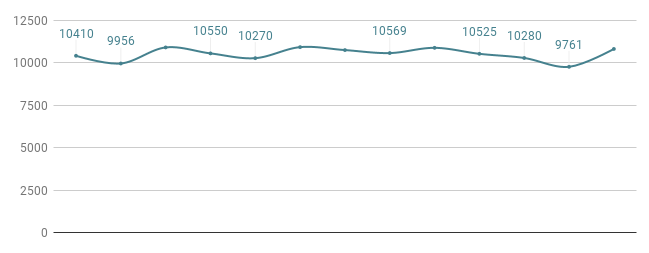
\includegraphics[width=0.9\textwidth]{sql-queries-psql}
\caption{Оцінка роботи обраної бази даних PostgreSQL}
\label{fig:sql-queries-psql}
\end{figure}

\begin{figure}[ht]
\centering
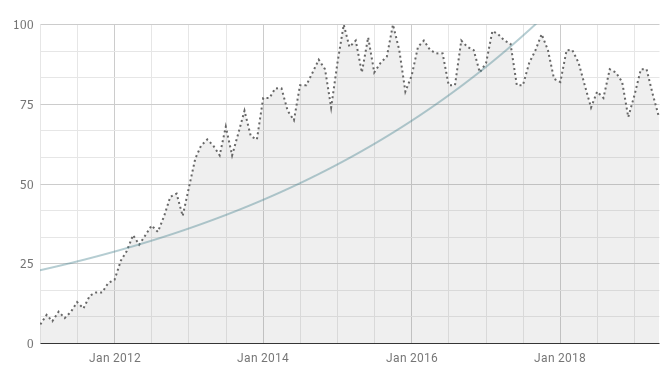
\includegraphics[width=0.8\textwidth]{big-data-search}
\caption{Тренд пошукових запитів із словосполученням «Big Data»}
\label{fig:big-data-search}
\end{figure}

\begin{figure}[ht]
\centering
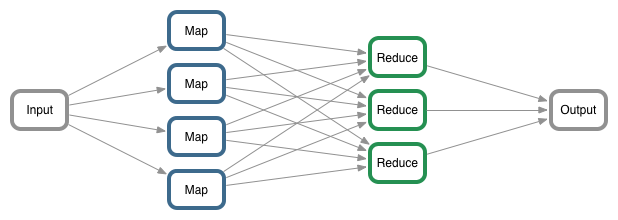
\includegraphics[width=0.8\textwidth]{map-reduce}
\caption{Схема роботи MapReduce}
\label{fig:map-reduce}
\end{figure}

\begin{figure}[ht]
\centering
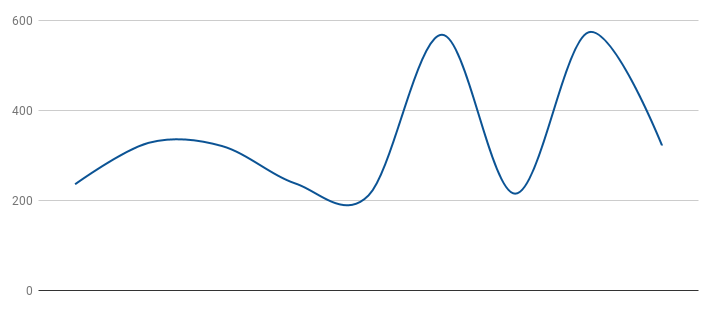
\includegraphics[width=0.8\textwidth]{opencars-service-performance}
\caption{Оцінка роботи розробленого веб-інтерфейсу}
\label{fig:opencars-service-performance}
\end{figure}

\begin{figure}[ht]
\centering
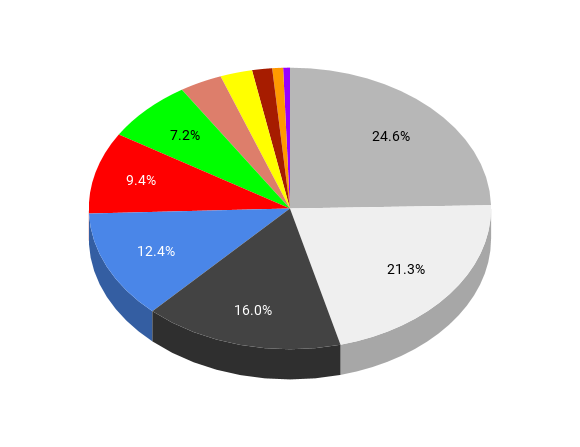
\includegraphics[width=0.5\textwidth]{transport-colors}
\caption{Розбиття кольорів Українського автотранспорту}
\label{fig:transport-colors}
\end{figure}

\chapter{}

\begin{figure}[h]
\centering
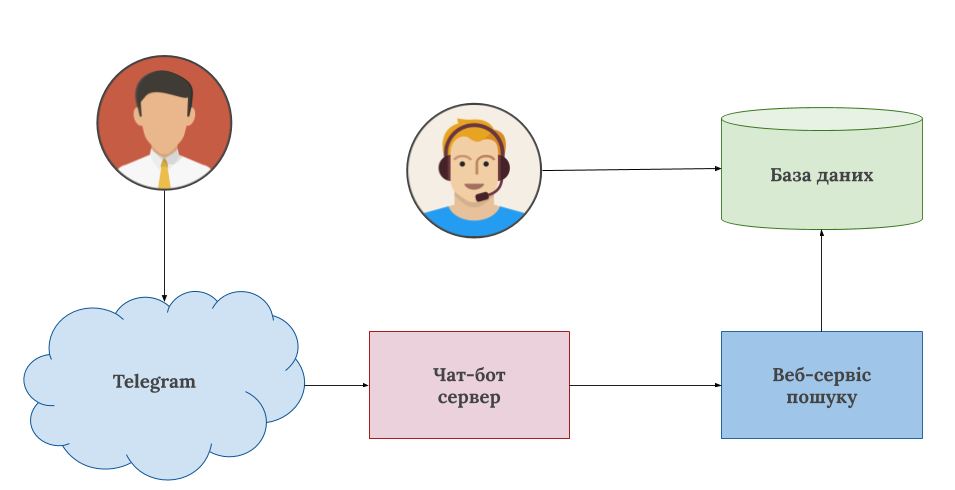
\includegraphics[width=0.5\textwidth]{user-system-overview}
\caption{Cхема роботи користувацької системи}
\label{fig:user-system-overview}
\end{figure}

\begin{figure}[h]
\centering
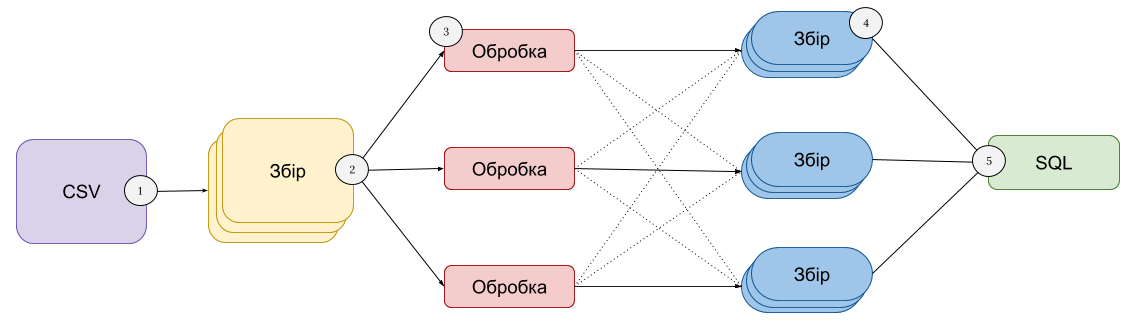
\includegraphics[width=0.7\textwidth]{parser-overview}
\caption{Обробка документів формату CSV у SQL}
\label{fig:parser-overview}
\end{figure}

\begin{figure}[h]
\centering
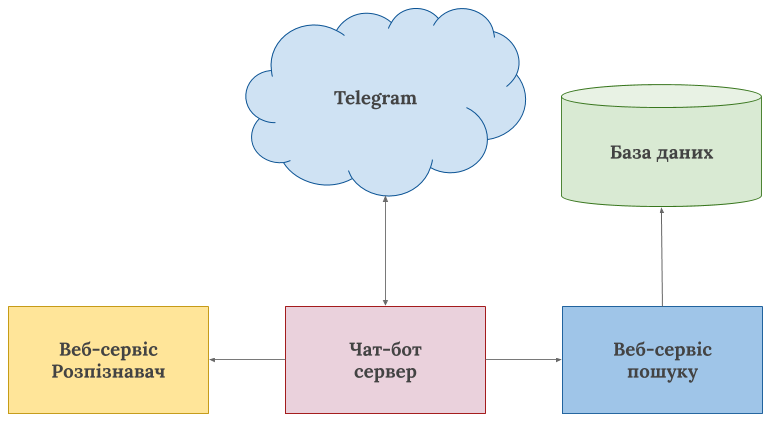
\includegraphics[width=0.5\textwidth]{architecture-overview}
\caption{Повна схема роботи системи}
\label{fig:architecture-overview}
\end{figure}


\end{document}
